\documentclass[11pt]{article}

% Add Graphics
\usepackage{graphicx, amsmath, hyperref}
\graphicspath{ {images/} }

% Set Section Counting to Start at 0
% \setcounter{section}{-1}

% Make better margins
	\addtolength{\oddsidemargin}{-.875in}
	\addtolength{\evensidemargin}{-.875in}
	\addtolength{\textwidth}{1.75in}

	\addtolength{\topmargin}{-.875in}
	\addtolength{\textheight}{1.75in}
	
\title{\textbf{YACS: Yet Another Cratering Simulation}}

\author{Tarek Mackler and Kyle Crabb}

\date{2016.12.01}

\begin{document}

\maketitle

\section*{An Overview}
It was this project's goal to simulate impact cratering of a 500km x 500km surface on a planet with no atmosphere. We aimed to simulate this scenario as realistically as possible, but simplifying assumptions were made.
\section{Cratering Simulation: Take One}

\subsection{Assumptions Made}
\textbf{Given assumptions:}
\begin{itemize}
	\item Crater Size: We are only considering craters larger than 10km
	\item Impact Parameters: We are only considering impacts close to \(90 ^{\circ} \), no secondary impact, and there is one impact per 1,000 years.
	\item Additional Given Assumptions: There are no outside factors that contribute to the addition or subtraction of craters, than the specified methods.
\end{itemize}
\textbf{Our assumptions:}
\begin{itemize}
	\item Impactor Size Distribution: To create a logarithmic distribution, our simulator takes the following process. First we generate discrete bin sizes that are logarithmic in amounts. Then we take a random, uniform distribution, and bias it with our bins. This provides a continuous distribution of impactors. We also set the simulation to ignore all craters smaller than 10km. 
	\item Crater Erasure: A crater is considered to be no longer visible once there are no more pixel of that crater visible. If even a single 1 km pixel is visible, that crater is counted.
	\item Surface Saturation: The surface is considered to be saturated once the original surface is no longer visible, that is to say, there are no more pixels of the original surface. If even a single 1km pixel is visible, the surface is unsaturated.
	\item Impactor vs Crater Size: We are only plotting crater sizes. As such it is more accurate to say that we are choosing Crater sizes and inferring impactor size from that.
	\item Saturation Limit: For the purposes of this simulation, we find saturation in the following way: After each impact, we take the average visible crater amount from the last 100 impacts and compare it to the last 1000. If the 100 average is within 1 \% of 1000 average, the surface is considered saturated.  
\end{itemize}

\subsection{Time Progression}
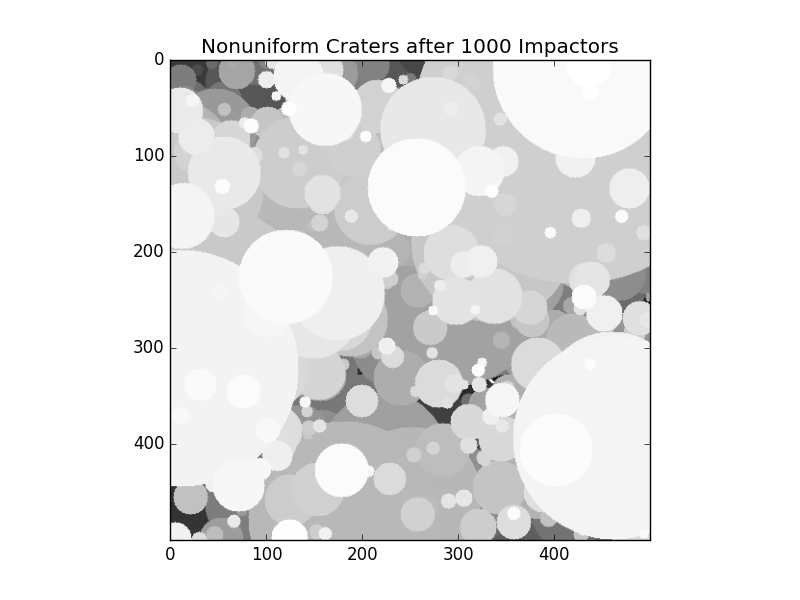
\includegraphics[scale=.4]{NonUniform1.png}
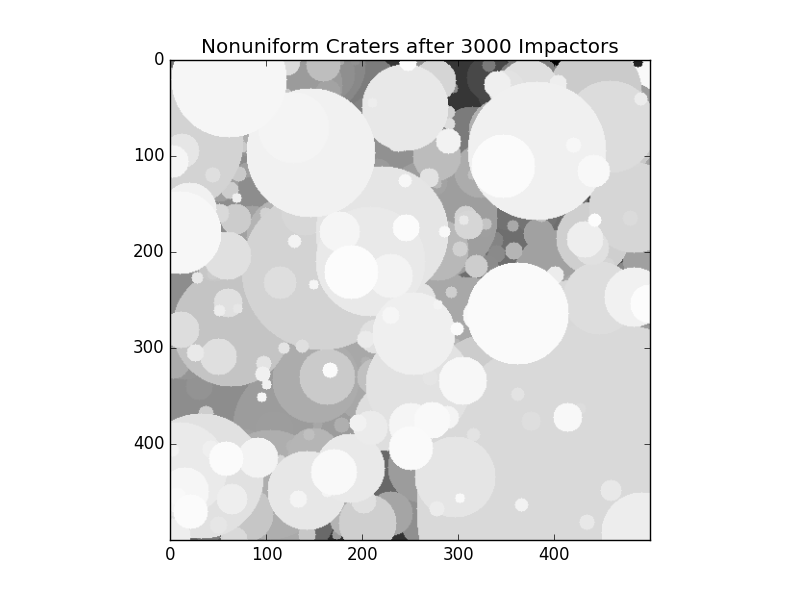
\includegraphics[scale=.4]{NonUniform3.png}\\
%\hspace{-4em}
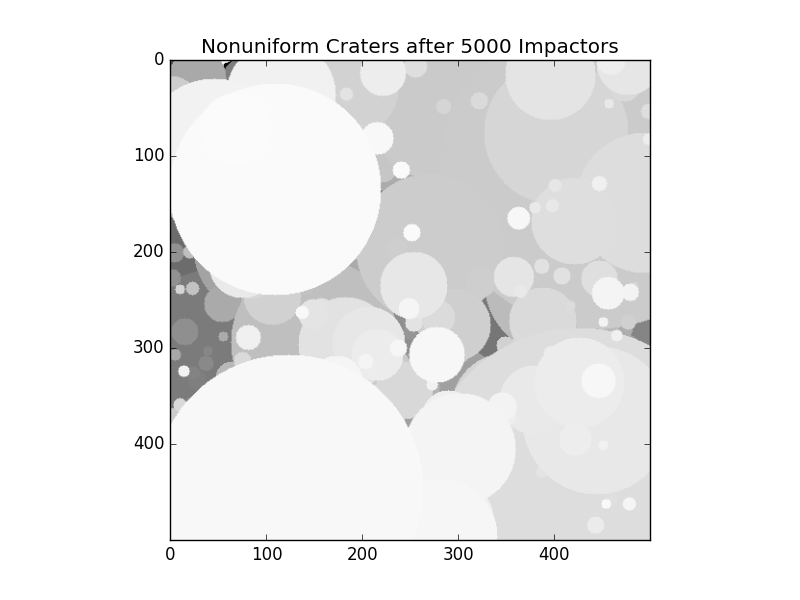
\includegraphics[scale=.4]{NonUniform5.png}
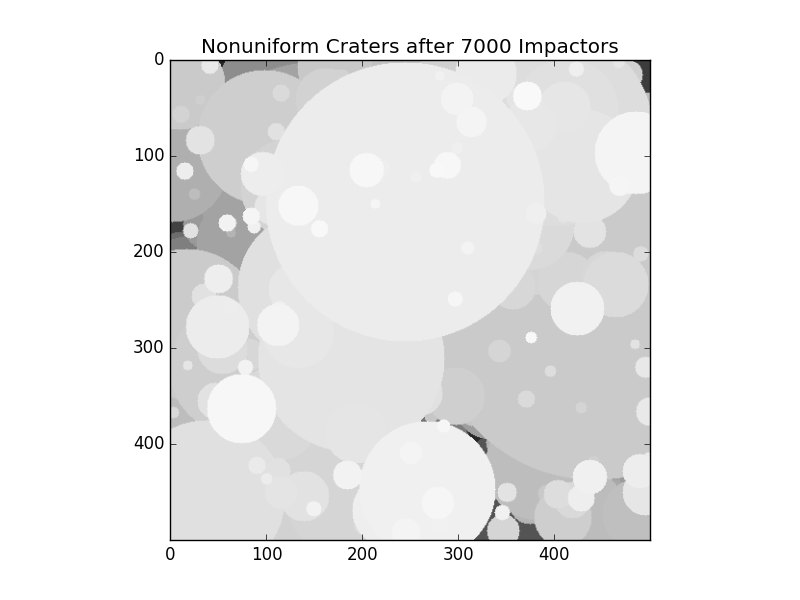
\includegraphics[scale=.4]{NonUniform7.png}\\
%\hspace{-4em}
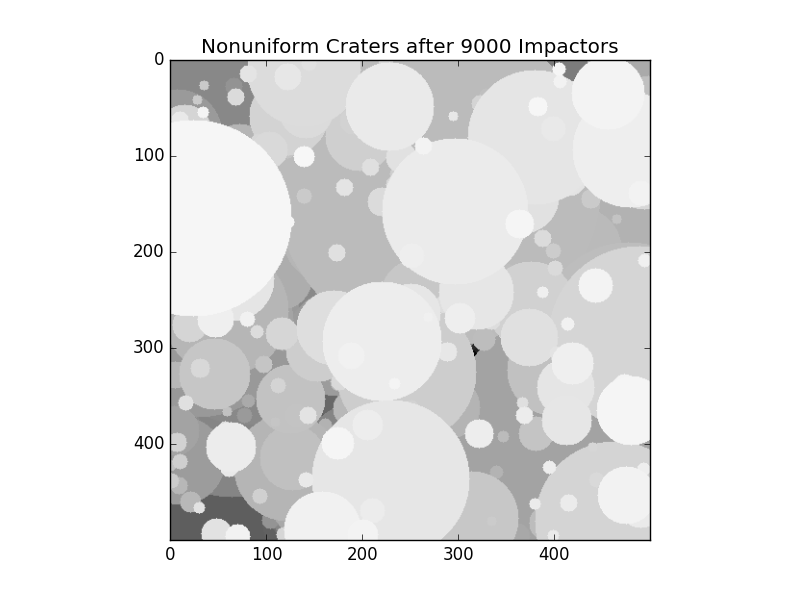
\includegraphics[scale=.4]{NonUniform9.png}
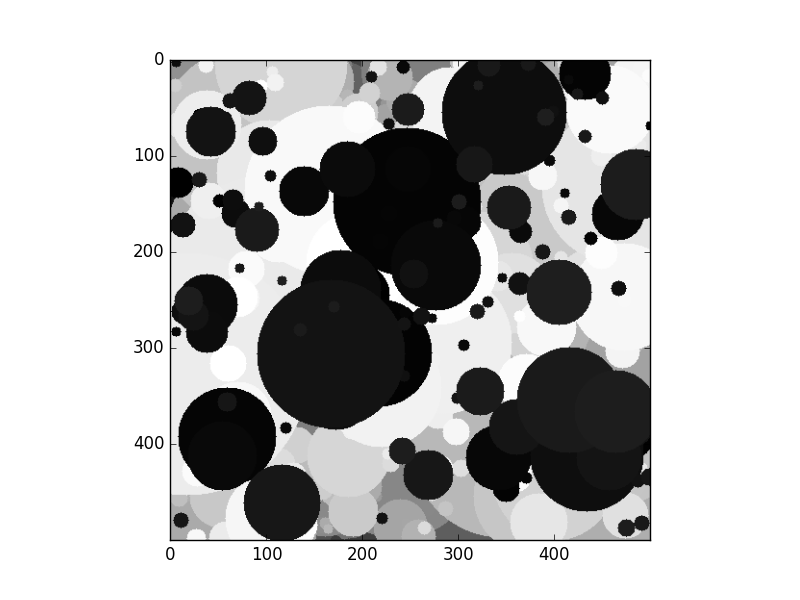
\includegraphics[scale=.4]{NonUniformSaturation.png}

\subsection{Visible Craters vs. Time}
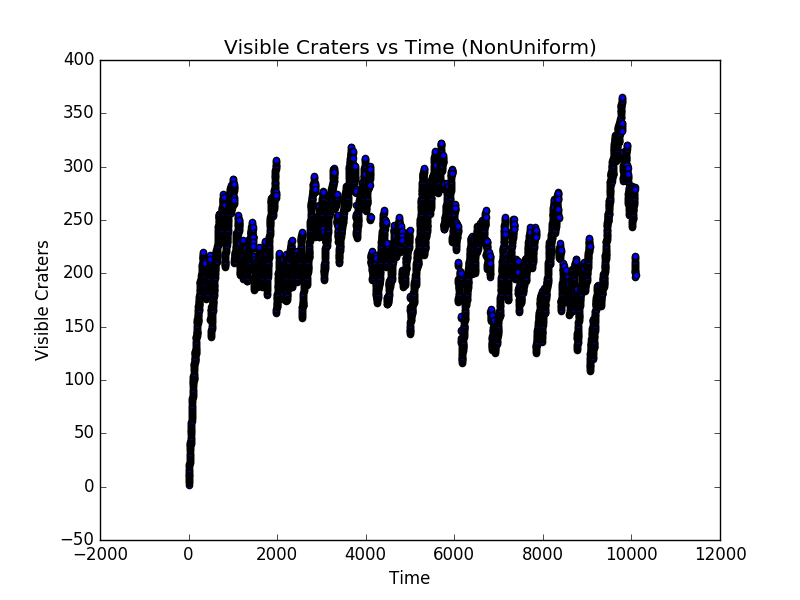
\includegraphics[scale=.85]{VisibleCratersvsTimeNonUniform.png}
\begin{center}
(Figure typo. x-axis label should read Time \( \left( \times 10^3 years \right) \)
\end{center}
\subsection{Analysis}

\subsubsection{Time Progression Analysis}
There are many fewer visible craters on the surface than there has been total impactors. Because of the varying size of craters, new craters have the potential to erase the evidence of many previous craters. A sufficiently large crater can cover more than half of the surface erasing most of the craters that existed. Additionally, smaller craters are easier to erase, since they have a smaller area. In our images, older craters are colored dark and newer craters are colored light. (Our colors rotate every 1000 impacts, which is the step amount. The last cratering image is "point of saturation" and not on the 1000 step scale. 
\subsubsection{Crater Visibility Analysis}
In the beginning, we see a quick rise, as the surface becomes impacted. Craters are created, but not very likely to be completely erased. We then see this level off, and the average increase is steady. Once this time has passed,  it has become more likely that a crater is overlapping another, and more time has passed to allow the chance of a large impactor to crater our surface, destroying numerous craters in the process. These large erasure events are visible in the large drops in visible crater count.

\section{Cratering Simulation: Take Two}

\subsection{Changed Assumption}
We also wished to examine what our simulation would produce if we assumed that all of the impactors were of the same size. All other assumptions have been kept the same.

\subsection{Time Progression}
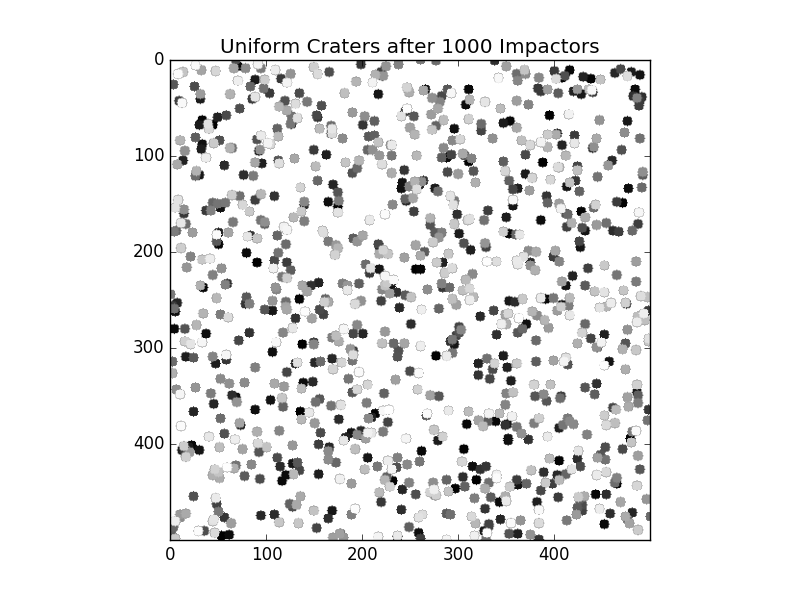
\includegraphics[scale=.4]{Uniform1.png}
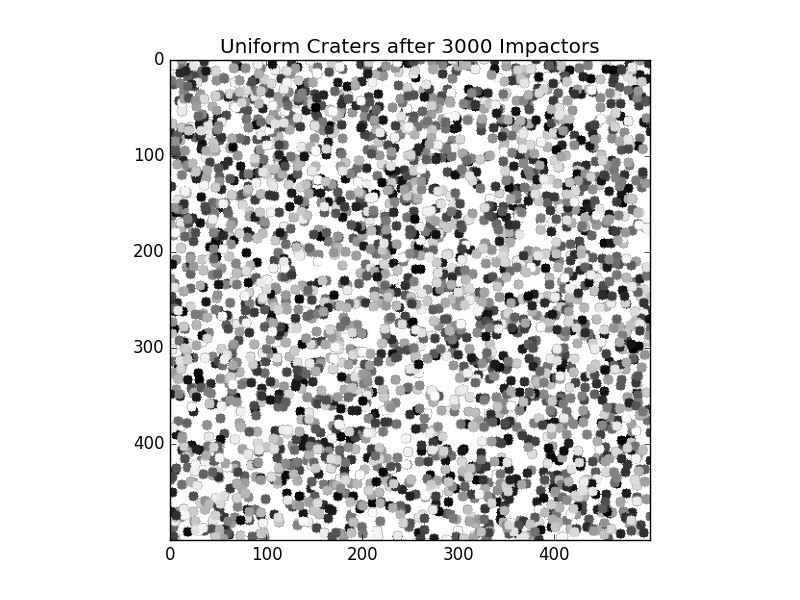
\includegraphics[scale=.4]{Uniform3.png}\\
%\hspace{-4em}
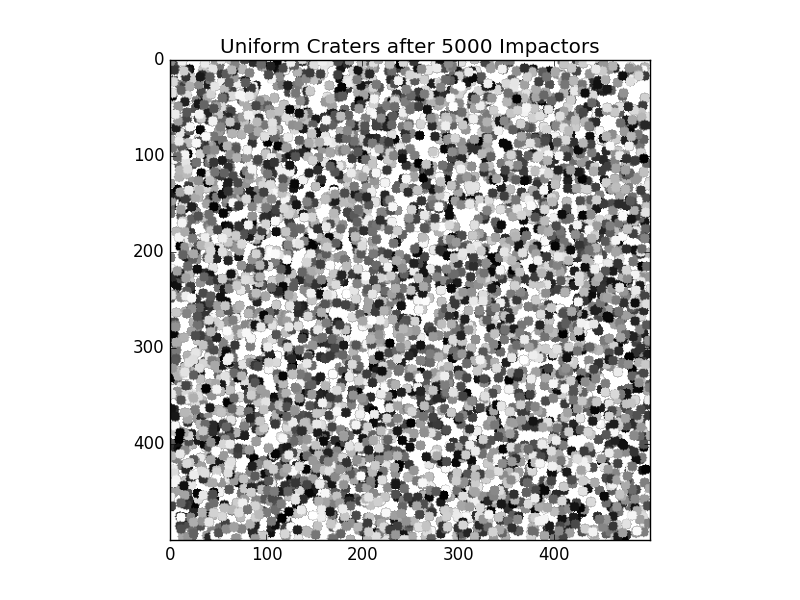
\includegraphics[scale=.4]{Uniform5.png}
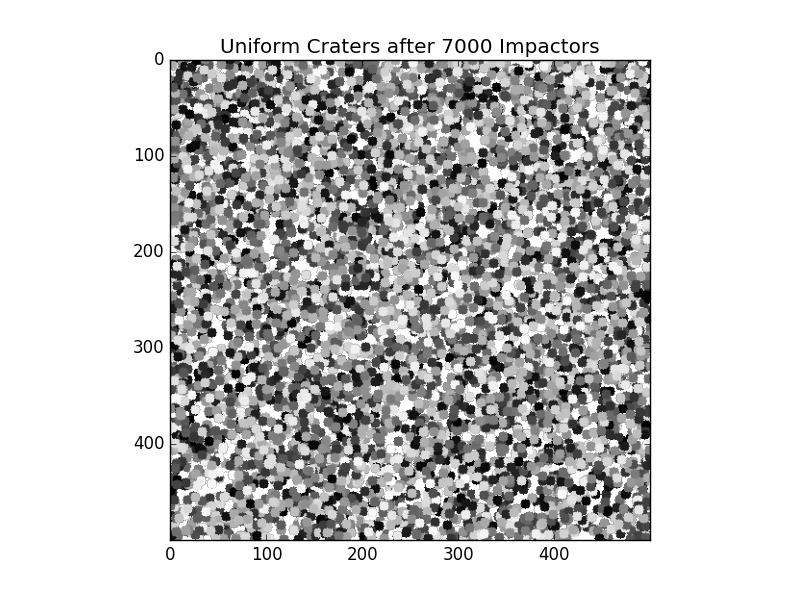
\includegraphics[scale=.4]{Uniform7.png}\\
%\hspace{-4em}
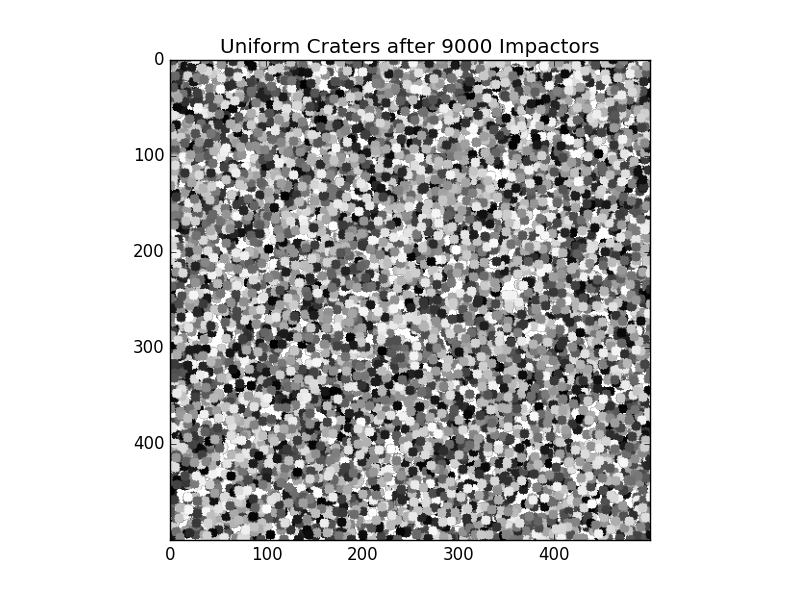
\includegraphics[scale=.4]{Uniform9.png}
\includegraphics[scale=.4]{UniformSaturation.png}

\subsection{Visible Craters vs. Time}
\includegraphics[scale=.85]{VisibleCratersvsTimeUniform.png}
\begin{center}
(Figure typo. x-axis label should read Time \( \left( \times 10^3 years \right) \)
\end{center}
\subsection{Analysis and Comparison to Non-Uniform}

\subsubsection{Time Progression Analysis}
Now, the craters look much more like static. They are all the same size, have the same probability of being erased, and erase the same amount of previous craters, so the craters all look very uniform and random (as a static screen is). 
 
\subsubsection{Crater Visibility Analysis}
Since the craters are much smaller and uniform this time around, there can exist many more on the surface without getting replaced. It would not be unreasonable to think that there could be 2500 complete craters at any time (think of a uniform 50 x 50 grid of 10km craters). This very linear progression to saturation makes sense because of this process. Another way to think about this is that, on average, if a crater does erase other craters, because of the uniform size, it will be around 1 crater erased on the impact. This is the definition of when a surface is saturated. Following our saturation guidelines, the flattening out happens at the end of the curve, compared to sooner, as seen with the Non-Uniform. If the curve continued, it would continue to flatten .

\section{Code}
Both codes can be found on our public \href{https://github.com/tkmr92/ASTR3750Project/tree/master/python}{\underline {\textit {Github Repository}}}(URL below). Our non-uniform distribution code is found under the file named \textit{crateringNonUniform.py} . Our uniform distribution code is found under the file named \textit{crateringUniform.py} . The code has also been included below. (To save on size, we have removed the comments. Comments can be seen in from the git files.)\\
\begin{center}
\underline{\textit{https://github.com/tkmr92/ASTR3750Project/tree/master/python/}}
\end{center}
\subsection{Non-Uniform Distribution}
\begin{verbatim}
import numpy as np
import matplotlib.pyplot as pl
import time
import sys

start = time.time()

image = np.zeros([500, 500, 4])

def genCratersize():
    bucket = np.random.logseries(0.8)
    cratersize = int(np.random.uniform(10*bucket, 20*bucket))
    return cratersize

def drawCircle(image, radius, origin, unique):
    xlim = int(radius)

    for i in range(origin[0] - xlim, origin[0] + (xlim + 1)):
        if (i > 499) or (i < 0):
            continue
        drawCalc = (radius * radius) - ((i-origin[0]) * (i-origin[0]))
        if drawCalc < 0:
            ylim = -int(( -drawCalc) ** .5)
        else:
            ylim = int( drawCalc ** .5)
        for j in range(origin[1] - ylim, origin[1] + (ylim + 1)):
            if (j > 499) or (j < 0):
                continue
            image[i][j][0] = unique
            image[i][j][1] = unique
            image[i][j][2] = unique
            image[i][j][3] = 1

    return(image)

def simImpacts(blankimage):

    count = 0
    unique = .001
    uniquelist = []
    cratersatstep = []
    cratermap = blankimage
    while True:
        if len(cratersatstep) > 10000:
            smallAvg = np.average(cratersatstep[-100:])
            bigAvg = np.average(cratersatstep[-1000:])
            if abs( smallAvg - bigAvg ) < (bigAvg * (1 - 0.99)):
                return cratermap, count, uniquelist, cratersatstep

        if count%1000 == 0:
            pl.imshow(image)
            pl.savefig('NonUniform'+str(count/1000)+'.png')
            pl.clf()

        impactsize = genCratersize()

        if impactsize < 10:
            continue
        count += 1

        x = int(np.random.rand()*500.)
        y = int(np.random.rand()*500.)

        cratermap = drawCircle(cratermap, int(impactsize / 2.), [x,y], unique)
        uniquelist = np.unique(cratermap[:,:,0])
        cratersatstep.append(len(uniquelist))

        unique += .001

    return cratermap, count, uniquelist, cratersatstep

image, totalcount, visible, cratercount = simImpacts(blankimage=image)

total = time.time() - start

print("""We have %i visible craters.
Our area saw %i impactors.
This equates to %.2e years taken to reach saturation.

This simulation took %f seconds to run.""" %(len(visible), totalcount, totalcount*1000, total))

pl.imshow(image)
pl.savefig('NonUniformSaturation.png')
pl.clf()

pl.scatter(np.linspace(0,len(cratercount), len(cratercount)), cratercount)
pl.xlabel('Time')
pl.ylabel('Visible Craters')
pl.title('Visible Craters vs Time')
pl.savefig('VisibleCratersvsTimeNonUniform.png')

\end{verbatim}

\subsection{Uniform Distribution}
\begin{verbatim}
import numpy as np
import matplotlib.pyplot as pl
import time

start = time.time()
image = np.zeros([500, 500, 4])

def drawCircle(image, radius, origin, unique):
    xlim = int(radius)
    for i in range(origin[0] - xlim, origin[0] + (xlim + 1)):
        if (i > (len(image) - 1)) or (i < 1):
            continue
        drawCalc = (radius * radius) - ((i-origin[0]) * (i-origin[0]))
        if drawCalc < 0:
            ylim = -int(( -drawCalc) ** .5)
        else:
            ylim = int( drawCalc ** .5)
        for j in range(origin[1] - ylim, origin[1] + (ylim + 1)):
            if (j > (len(image) - 1)) or (j < 1):
                continue
            image[i][j][0] = unique
            image[i][j][1] = unique
            image[i][j][2] = unique
            image[i][j][3] = 1
    return(image)

def simImpacts(blankimage):
    count = 0
    unique = .001
    uniquelist = []
    cratersatstep = []
    cratermap = blankimage

    while True:
        if len(cratersatstep) > 10000:
            smallAvg = np.average(cratersatstep[-100:])
            bigAvg = np.average(cratersatstep[-1000:])
            if abs( smallAvg - bigAvg ) < (bigAvg * (1 - 0.99)):
                return cratermap, count, uniquelist, cratersatstep

        if count%1000 == 0:
            pl.imshow(image)
            pl.title('Uniform Craters after '+str(int(count))+' Impactors')
            pl.savefig('../images/Uniform'+str(int(count/1000))+'.png')
            pl.clf()

        count += 1
        x = int(np.random.rand()*500.)
        y = int(np.random.rand()*500.)
        impactsize = 10
        cratermap = drawCircle(cratermap, int(impactsize / 2.), [x,y], unique)
        uniquelist = np.unique(cratermap[:,:,0])
        cratersatstep.append(len(uniquelist))
        unique += .001
     return cratermap, count , uniquelist, cratersvisible

image, totalcount, visible, cratercount = simImpacts(blankimage=image)

total = time.time() - start
print("""We have %i visible craters.
Our area saw %i impacters.
This equates to %.2e years taken to reach saturation.

This simulation took %f seconds to run.""" %(len(visible), totalcount, totalcount*1000, total))

pl.imshow(image)
pl.savefig("../images/uniformSaturation.png")
pl.title('Craters at Saturation')
pl.clf()

pl.scatter(np.linspace(0,len(cratercount), len(cratercount)), cratercount)
pl.xlabel('Time')
pl.ylabel('Visible Craters')
pl.title('Visible Craters vs Time (Uniform)')
pl.savefig('../images/VisiblecratersvsTimeUniform.png')

\end{verbatim}

\end{document}